\documentclass[11pt]{article}
\usepackage[notes]{la}
\lamodule{2}{5}{Matrix Factorizations}
\laxdoc{1.2}
\laxdoc{2.1}
\laxdoc{2.2}

\begin{document}

\section{Matrix Factorizations}

\begin{guide}
Row reduction is a one-way street: it starts with $A$, ends with an echelon form, and forgets every step along the way. Suppose, though, that the \emph{same} matrix $A$ must be used with a thousand different right-hand sides $\bv{b}$. Must we repeat the whole elimination a thousand times? Can the steps be \emph{remembered}, in a form that is cheap to store and cheap to reuse? And what exactly goes wrong when a row interchange is needed?
\end{guide}

\begin{remark}[About this section]
This section is enrichment: it is not on the exams, and its homework is optional. It uses nothing beyond Chapter~1 and Sections 2.1 and 2.2, and it rewards a careful reader, because it shows that the elementary matrices of Section~2.2 are more than a proof device.
\end{remark}

\textbf{By the end of this section you should be able to:}
\begin{itemize}
  \item explain why an $LU$ factorization is ``row reduction remembered'': $U$ is the echelon form, $L$ is the record of the steps;
  \item find an $LU$ factorization of a matrix (square or not) by forward elimination, filling in $L$ directly from the multipliers;
  \item solve $A\bv{x}=\bv{b}$ with $L$ and $U$ by forward and back substitution, and say why this pays off when $A$ is reused;
  \item decide whether a matrix has an $LU$ factorization, and explain what a row interchange does to the factorization (the permuted $LU$ factorization $PA=LU$);
  \item decide, from the elimination, \emph{where} and \emph{why} an $LU$ factorization fails without a row swap.
\end{itemize}

% ---------------------------------------------------------------------
\subsection*{Triangular matrices and the shape of a factorization}

A \emph{factorization} writes a matrix as a product of simpler matrices, the way $60=4\cdot3\cdot5$ writes a number as a product of simpler numbers. ``Simpler'' here will mean \emph{triangular}.

\begin{defn}{Triangular matrices}{triangular}
A square matrix is \emph{lower triangular} if all of its entries above the diagonal are $0$, and \emph{upper triangular} if all of its entries below the diagonal are $0$. A lower triangular matrix is \emph{unit lower triangular} if, in addition, every diagonal entry is $1$.
\end{defn}

\begin{defn}{LU factorization}{lu}
Let $A$ be an $m\times n$ matrix. An \emph{$LU$ factorization} of $A$ is an equation
\[
A=LU,
\]
where $L$ is an $m\times m$ unit lower triangular matrix and $U$ is an $m\times n$ echelon form of $A$. (Because an echelon form has only zeros below its staircase, $U$ plays the role of ``upper triangular'' even when it is not square.)
\end{defn}

\begin{center}
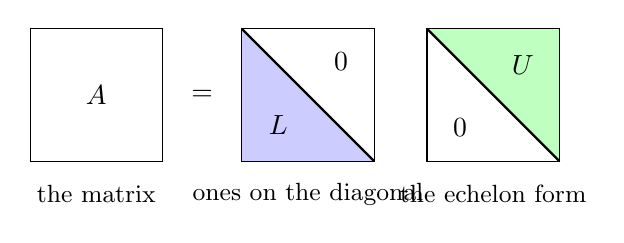
\begin{tikzpicture}[scale=0.42,>=stealth]
  \begin{scope}
    \draw (0,0) rectangle (4,4);
    \node at (2,2) {$A$};
    \node at (2,-1.0) {\small the matrix};
  \end{scope}
  \node at (5.2,2) {$=$};
  \begin{scope}[xshift=6.4cm]
    \fill[blue!20] (0,4)--(0,0)--(4,0)--cycle;
    \draw (0,0) rectangle (4,4);
    \draw[thick] (0,4)--(4,0);
    \node at (1.1,1.1) {$L$};
    \node at (3.0,3.0) {0};
    \node at (2,-1.0) {\small ones on the diagonal};
  \end{scope}
  \begin{scope}[xshift=12cm]
    \fill[green!25] (0,4)--(4,4)--(4,0)--cycle;
    \draw (0,0) rectangle (4,4);
    \draw[thick] (0,4)--(4,0);
    \node at (2.9,2.9) {$U$};
    \node at (1.0,1.0) {0};
    \node at (2,-1.0) {\small the echelon form};
  \end{scope}
\end{tikzpicture}
\end{center}

\textbf{Figure.} The shape of $A=LU$ for a square matrix. The factor $L$ has zeros above its diagonal and ones on it; the factor $U$ has zeros below its diagonal. Everything interesting about $L$ lives in the shaded triangle \emph{below} the diagonal.

\begin{kc}{Which kind of triangular?}{triangular}
Classify each matrix as lower triangular, upper triangular, unit lower triangular, or none of these (more than one answer may apply):
\[
\text{(a)}\begin{bmatrix}1&0&0\\4&1&0\\-2&5&1\end{bmatrix}\quad
\text{(b)}\begin{bmatrix}3&0\\1&2\end{bmatrix}\quad
\text{(c)}\begin{bmatrix}1&2\\0&1\end{bmatrix}\quad
\text{(d)}\begin{bmatrix}1&0\\0&1\end{bmatrix}\quad
\text{(e)}\begin{bmatrix}1&0&2\\3&1&0\\0&0&1\end{bmatrix}
\]
\end{kc}

% ---------------------------------------------------------------------
\subsection*{Row reduction, remembered}

The key observation is already in Section~2.2. Each row operation is multiplication on the left by an elementary matrix (Theorem~\ref{2.2-thm:elementary}), and each elementary matrix has an inverse that undoes it. Let us see what this says when only the simplest kind of step is used.

\begin{exmp}{One step, remembered}{onestep}
Let $A=\begin{bmatrix}2&1\\6&4\end{bmatrix}$. The single step $R_2-3R_1\to R_2$ reaches an echelon form:
\[
\begin{bmatrix}2&1\\6&4\end{bmatrix}\rops{R_2-3R_1}\begin{bmatrix}2&1\\0&1\end{bmatrix}=U .
\]
In matrix language this step is $EA=U$ with $E=\begin{bmatrix}1&0\\-3&1\end{bmatrix}$. Multiply both sides on the left by $E^{-1}=\begin{bmatrix}1&0\\3&1\end{bmatrix}$ (the reverse step, Theorem~\ref{2.2-thm:elementary}(b)):
\[
A=E^{-1}U,\qquad\text{that is,}\qquad
\begin{bmatrix}1&0\\3&1\end{bmatrix}\begin{bmatrix}2&1\\0&1\end{bmatrix}=\begin{bmatrix}2&1\\6&4\end{bmatrix}.
\]
So $L=E^{-1}$. Notice where the $3$ sits: row operation ``subtract $3$ times row~1 from row~2'' left a $3$ in position $(2,1)$ of $L$. The factor $L$ \emph{is} the log of the elimination: it says ``to get $A$ back from $U$, add $3$ times row~1 to row~2.''
\end{exmp}

A longer elimination uses several steps, and the matrices multiply.

\begin{exmp}{A $3\times3$ factorization from elementary matrices}{threeE}
Let $A=\begin{bmatrix}2&1&1\\6&4&5\\4&1&3\end{bmatrix}$. Forward elimination, using only replacements:
\begin{align*}
\begin{bmatrix}2&1&1\\6&4&5\\4&1&3\end{bmatrix}
&\rops{R_2-3R_1,\ R_3-2R_1}
\begin{bmatrix}2&1&1\\0&1&2\\0&-1&1\end{bmatrix}
\rops{R_3+R_2}
\begin{bmatrix}2&1&1\\0&1&2\\0&0&3\end{bmatrix}=U .
\end{align*}
There are three steps, so three elementary matrices:
\[
E_1=\begin{bmatrix}1&0&0\\-3&1&0\\0&0&1\end{bmatrix},\quad
E_2=\begin{bmatrix}1&0&0\\0&1&0\\-2&0&1\end{bmatrix},\quad
E_3=\begin{bmatrix}1&0&0\\0&1&0\\0&1&1\end{bmatrix},
\]
for $R_2-3R_1$, $R_3-2R_1$ and $R_3+R_2$, in that order. Then $E_3E_2E_1A=U$; checking it by multiplication:
\[
\begin{bmatrix}1&0&0\\0&1&0\\0&1&1\end{bmatrix}
\begin{bmatrix}1&0&0\\0&1&0\\-2&0&1\end{bmatrix}
\begin{bmatrix}1&0&0\\-3&1&0\\0&0&1\end{bmatrix}
\begin{bmatrix}2&1&1\\6&4&5\\4&1&3\end{bmatrix}
=\begin{bmatrix}2&1&1\\0&1&2\\0&0&3\end{bmatrix}.
\]
Solving for $A$ gives $A=E_1^{-1}E_2^{-1}E_3^{-1}U$, and each inverse is the reverse step:
\[
\begin{bmatrix}1&0&0\\3&1&0\\0&0&1\end{bmatrix}
\begin{bmatrix}1&0&0\\0&1&0\\2&0&1\end{bmatrix}
\begin{bmatrix}1&0&0\\0&1&0\\0&-1&1\end{bmatrix}
=\begin{bmatrix}1&0&0\\3&1&0\\2&-1&1\end{bmatrix}=L .
\]
Look at $L$. It is unit lower triangular, and its entries below the diagonal are the multipliers $3$, $2$ and $-1$, each placed at the position it eliminated, with the sign reversed relative to the row operation ($R_3+R_2$ is $R_3-(-1)R_2$). Check the whole factorization:
\[
\begin{bmatrix}1&0&0\\3&1&0\\2&-1&1\end{bmatrix}
\begin{bmatrix}2&1&1\\0&1&2\\0&0&3\end{bmatrix}
=\begin{bmatrix}2&1&1\\6&4&5\\4&1&3\end{bmatrix}=A.\ \checkmark
\]
\end{exmp}

\begin{think}{Why do the multipliers land in $L$ untouched?}{mixing}
In Example~\ref{ex:threeE} the matrix that \emph{reduces} $A$ is $E_3E_2E_1$, and the matrix that \emph{rebuilds} it is $L=E_1^{-1}E_2^{-1}E_3^{-1}$. Multiply out $E_3E_2E_1$. Do the numbers $3$, $2$ and $-1$ appear in it as they appear in $L$? Why is the product of the inverses so much tidier than the product of the originals?
\end{think}

The tidiness is no accident. It holds for every forward elimination done in the usual order, and the proof is short.

\begin{thm}{The multipliers fill in $L$}{multipliers}
Let $A$ be an $m\times n$ matrix, and suppose forward elimination reduces $A$ to an echelon form $U$ using only replacements of the form
\[
R_i-\ell_{ik}R_k\to R_i\qquad(i>k),
\]
where $R_k$ is the $k$th pivot row, performed pivot by pivot from the top: first all the replacements that use pivot row~$1$, then all those that use pivot row~$2$, and so on. Let $L$ be the $m\times m$ matrix with $1$ on every diagonal position, the multiplier $\ell_{ik}$ in position $(i,k)$ for every replacement used, and $0$ in every other position. Then $A=LU$.
\end{thm}

\begin{proof}
All replacements that use pivot row $k$ can be carried out together by one matrix $G_k=I-N_k$, where $N_k$ has the entry $\ell_{ik}$ in position $(i,k)$ for each $i>k$ and zeros elsewhere (only column $k$ of $N_k$ is nonzero, and only below the diagonal). Then $G_r\cdots G_2G_1A=U$, where $r$ is the number of pivots.

The entry in position $(i,j)$ of a product $N_aN_b$ is $\sum_t(N_a)_{it}(N_b)_{tj}$. A term of this sum can be nonzero only if $(N_a)_{it}\neq0$, which forces $t=a$ (the only nonzero entries of $N_a$ are in column $a$), and $(N_b)_{tj}\neq0$, which forces $t>b$ (the only nonzero entries of $N_b$ are below row $b$). Both requirements can hold only when $a>b$. Hence $N_aN_b=0$ whenever $a\le b$; in particular $N_kN_k=0$, so $(I-N_k)(I+N_k)=I-N_kN_k=I$ and $G_k^{-1}=I+N_k$. Hence
\[
G_1^{-1}G_2^{-1}\cdots G_r^{-1}=(I+N_1)(I+N_2)\cdots(I+N_r)=I+N_1+N_2+\cdots+N_r ,
\]
because every product $N_aN_b$ with $a<b$ vanishes (the factors appear in increasing order of their indices). The right-hand side is exactly the matrix $L$ of the theorem, and $A=G_1^{-1}\cdots G_r^{-1}U=LU$.
\end{proof}

\begin{proc}{Finding an $LU$ factorization}{lu}
\begin{enumerate}
  \item Reduce $A$ to an echelon form $U$ using only replacements $R_i-\ell R_k\to R_i$ with $i>k$ (add a multiple of a row to a row \emph{below} it), working down the pivot columns from left to right. If you are ever forced to interchange rows, stop: see the last part of this section.
  \item Start with $L=I_m$. Every time you use $R_i-\ell R_k\to R_i$, write the multiplier $\ell$ in position $(i,k)$ of $L$. (The multiplier is the entry you are eliminating divided by the pivot.)
  \item Check at least one entry of $LU$ against $A$.
\end{enumerate}
\end{proc}

\begin{warn}[Mind the sign]
The row operation $R_3+2R_1\to R_3$ eliminates by \emph{adding}, so its multiplier is $\ell_{31}=-2$, and $L$ gets the entry $-2$. The entry of $L$ is the multiplier $\ell$ in $R_i-\ell R_k$, never the number written next to the plus sign.
\end{warn}

\begin{exmp}{Fractions among the multipliers}{fractions}
Find an $LU$ factorization of $A=\begin{bmatrix}2&4&6\\1&5&4\\-2&2&-2\end{bmatrix}$.

\textbf{Solution.} The pivot in position $(1,1)$ is $2$. To clear the $1$ below it we subtract $\tfrac12$ of row~$1$; to clear the $-2$ we add row~$1$ (multiplier $-1$):
\begin{align*}
\begin{bmatrix}2&4&6\\1&5&4\\-2&2&-2\end{bmatrix}
&\rops{R_2-\frac12R_1,\ R_3+R_1}
\begin{bmatrix}2&4&6\\0&3&1\\0&6&4\end{bmatrix}
\rops{R_3-2R_2}
\begin{bmatrix}2&4&6\\0&3&1\\0&0&2\end{bmatrix}=U .
\end{align*}
The multipliers are $\ell_{21}=\tfrac12$, $\ell_{31}=-1$ and $\ell_{32}=2$, so
\[
L=\begin{bmatrix}1&0&0\\\tfrac12&1&0\\-1&2&1\end{bmatrix},\qquad
\begin{bmatrix}1&0&0\\\tfrac12&1&0\\-1&2&1\end{bmatrix}\begin{bmatrix}2&4&6\\0&3&1\\0&0&2\end{bmatrix}=\begin{bmatrix}2&4&6\\1&5&4\\-2&2&-2\end{bmatrix}.\ \checkmark
\]
The fractions come only from dividing by pivots, and they live in $L$; the pivots $2$, $3$, $2$ sit on the diagonal of $U$.
\end{exmp}

\begin{kc}{Fill in $L$}{fillL}
A $3\times3$ matrix is reduced to an echelon form by the steps $R_2-4R_1\to R_2$, then $R_3+2R_1\to R_3$, then $R_3-5R_2\to R_3$. Without knowing the matrix, write down the matrix $L$ in its $LU$ factorization.
\end{kc}

\begin{kc}{Elementary matrices and their inverses}{inverseE}
Write the $3\times3$ elementary matrix $E$ of the step $R_3-2R_2\to R_3$ and its inverse $E^{-1}$. Is each of them unit lower triangular?
\end{kc}

% ---------------------------------------------------------------------
\subsection*{A $4\times4$ example, by hand}

Nothing in the procedure depends on size, only on patience. Here is a complete $4\times4$ example, done the way you would do it on paper.

\begin{exmp}{An $LU$ factorization of a $4\times4$ matrix}{fourbyfour}
Factor
\[
A=\begin{bmatrix}2&1&0&3\\4&3&2&7\\-2&2&9&2\\2&-1&-1&5\end{bmatrix}.
\]

\textbf{Step 1: column 1.} The pivot is the $2$ in position $(1,1)$. The entries below it are $4$, $-2$, $2$, so the multipliers are $\ell_{21}=2$, $\ell_{31}=-1$, $\ell_{41}=1$.

\textbf{Step 2: column 2.} In the new matrix the pivot is the $1$ in position $(2,2)$ and the entries below it are $3$ and $-2$, so $\ell_{32}=3$ and $\ell_{42}=-2$.

\textbf{Step 3: column 3.} The pivot is the $3$ in position $(3,3)$, the entry below it is $3$, so $\ell_{43}=1$.

All three steps in one chain:
\begin{align*}
\begin{bmatrix}2&1&0&3\\4&3&2&7\\-2&2&9&2\\2&-1&-1&5\end{bmatrix}
&\rops{R_2-2R_1,\ R_3+R_1,\ R_4-R_1}
\begin{bmatrix}2&1&0&3\\0&1&2&1\\0&3&9&5\\0&-2&-1&2\end{bmatrix}\\[4pt]
&\rops{R_3-3R_2,\ R_4+2R_2}
\begin{bmatrix}2&1&0&3\\0&1&2&1\\0&0&3&2\\0&0&3&4\end{bmatrix}
\rops{R_4-R_3}
\begin{bmatrix}2&1&0&3\\0&1&2&1\\0&0&3&2\\0&0&0&2\end{bmatrix}=U .
\end{align*}
Collect the multipliers, column by column, below the diagonal of an identity matrix:
\[
L=\begin{bmatrix}1&0&0&0\\2&1&0&0\\-1&3&1&0\\1&-2&1&1\end{bmatrix}.
\]
\textbf{Check.} Multiply $L$ by $U$:
\[
\begin{bmatrix}1&0&0&0\\2&1&0&0\\-1&3&1&0\\1&-2&1&1\end{bmatrix}
\begin{bmatrix}2&1&0&3\\0&1&2&1\\0&0&3&2\\0&0&0&2\end{bmatrix}
=\begin{bmatrix}2&1&0&3\\4&3&2&7\\-2&2&9&2\\2&-1&-1&5\end{bmatrix}.\ \checkmark
\]
Two quick checks catch most slips: the first row of $A$ equals the first row of $U$ (row~$1$ is never changed), and the first column of $A$ equals $u_{11}=2$ times the first column of $L$: $2\cdot(1,2,-1,1)=(2,4,-2,2)$.
\end{exmp}

\begin{kc}{Two quick checks}{twochecks}
In Example~\ref{ex:fourbyfour}, what are the pivots, and where do they appear? What is the second column of $A$ in terms of the columns of $L$ and the second column of $U$? (Hint: the $j$th column of $LU$ is $L$ times the $j$th column of $U$.)
\end{kc}

\begin{exmp}{A matrix that is not square}{rect}
Find an $LU$ factorization of $A=\begin{bmatrix}1&2&-1&3\\2&4&1&0\\-1&-2&4&-7\end{bmatrix}$.

\textbf{Solution.} Here $L$ is $3\times3$ and $U$ is $3\times4$. Column~2 has no pivot after clearing column~1, so the second pivot is in column~3:
\begin{align*}
\begin{bmatrix}1&2&-1&3\\2&4&1&0\\-1&-2&4&-7\end{bmatrix}
&\rops{R_2-2R_1,\ R_3+R_1}
\begin{bmatrix}1&2&-1&3\\0&0&3&-6\\0&0&3&-4\end{bmatrix}
\rops{R_3-R_2}
\begin{bmatrix}1&2&-1&3\\0&0&3&-6\\0&0&0&2\end{bmatrix}=U .
\end{align*}
The multipliers are $\ell_{21}=2$, $\ell_{31}=-1$ and $\ell_{32}=1$. The second pivot row is row~$2$ (the \emph{row} number of the pivot, not the column number $3$, decides where the multiplier goes), so
\[
L=\begin{bmatrix}1&0&0\\2&1&0\\-1&1&1\end{bmatrix},\qquad
\begin{bmatrix}1&0&0\\2&1&0\\-1&1&1\end{bmatrix}\begin{bmatrix}1&2&-1&3\\0&0&3&-6\\0&0&0&2\end{bmatrix}=\begin{bmatrix}1&2&-1&3\\2&4&1&0\\-1&-2&4&-7\end{bmatrix}.\ \checkmark
\]
\end{exmp}

% ---------------------------------------------------------------------
\subsection*{Solving $A\bv{x}=\bv{b}$ with $L$ and $U$}

Why do we want $A=LU$? Because both factors are easy to solve with. Suppose $A=LU$ and we must solve $A\bv{x}=\bv{b}$. Replace $A$ by $LU$:
\[
L(U\bv{x})=\bv{b}.
\]
Give the unknown vector $U\bv{x}$ a name, $\bv{y}$. Then we have two systems to solve, one after the other.

\begin{thm}{Solving with $LU$}{lusolve}
Let $A=LU$ with $L$ unit lower triangular and $U$ in echelon form. Then $\bv{x}$ solves $A\bv{x}=\bv{b}$ if and only if there is a vector $\bv{y}$ such that
\[
L\bv{y}=\bv{b}\qquad\text{and}\qquad U\bv{x}=\bv{y}.
\]
\end{thm}

\begin{proof}
If $L\bv{y}=\bv{b}$ and $U\bv{x}=\bv{y}$, then $A\bv{x}=L(U\bv{x})=L\bv{y}=\bv{b}$ by associativity (Theorem~\ref{2.1-thm:mulprops}). Conversely, if $A\bv{x}=\bv{b}$, take $\bv{y}=U\bv{x}$; then $L\bv{y}=LU\bv{x}=\bv{b}$.
\end{proof}

The first system, $L\bv{y}=\bv{b}$, is solved from the top down (\emph{forward substitution}): the first equation says $y_1=b_1$ because $L$ has a $1$ on the diagonal and nothing else in row~$1$; the second involves only $y_1$ and $y_2$; and so on. No division is needed, because the diagonal entries are $1$. The second system, $U\bv{x}=\bv{y}$, is solved from the bottom up (\emph{back substitution}), exactly as at the end of Section~1.2.

\begin{center}
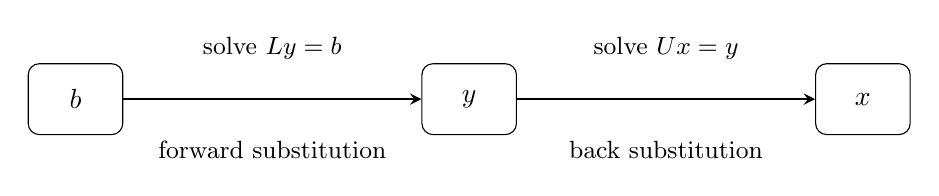
\begin{tikzpicture}[>=stealth]
  \node[draw,rounded corners,minimum width=1.2cm,minimum height=0.9cm] (b) at (0,0) {$b$};
  \node[draw,rounded corners,minimum width=1.2cm,minimum height=0.9cm] (y) at (5,0) {$y$};
  \node[draw,rounded corners,minimum width=1.2cm,minimum height=0.9cm] (x) at (10,0) {$x$};
  \draw[->,thick] (b)--(y);
  \draw[->,thick] (y)--(x);
  \node at (2.5,0.65) {\small solve $Ly=b$};
  \node at (2.5,-0.65) {\small forward substitution};
  \node at (7.5,0.65) {\small solve $Ux=y$};
  \node at (7.5,-0.65) {\small back substitution};
\end{tikzpicture}
\end{center}

\textbf{Figure.} The two triangular solves that replace one full elimination. Both are quick, because each equation has only one new unknown.

\begin{exmp}{Solving with $L$ and $U$ given}{givenLU}
Let $A=LU$ with
\[
L=\begin{bmatrix}1&0&0\\2&1&0\\-1&3&1\end{bmatrix},\qquad U=\begin{bmatrix}1&-2&3\\0&2&-1\\0&0&4\end{bmatrix},\qquad \bv{b}=\begin{bmatrix}-3\\-3\\8\end{bmatrix}.
\]
Solve $A\bv{x}=\bv{b}$.

\textbf{Solution.} First $L\bv{y}=\bv{b}$. Reducing $[\,L\mid\bv{b}\,]$ with replacements is forward substitution:
\begin{align*}
\begin{amat}{ccc|c}1&0&0&-3\\2&1&0&-3\\-1&3&1&8\end{amat}
&\rops{R_2-2R_1,\ R_3+R_1}
\begin{amat}{ccc|c}1&0&0&-3\\0&1&0&3\\0&3&1&5\end{amat}
\rops{R_3-3R_2}
\begin{amat}{ccc|c}1&0&0&-3\\0&1&0&3\\0&0&1&-4\end{amat},
\end{align*}
so $\bv{y}=(-3,3,-4)$. Now $U\bv{x}=\bv{y}$, by back substitution:
\begin{align*}
\begin{amat}{ccc|c}1&-2&3&-3\\0&2&-1&3\\0&0&4&-4\end{amat}
&\rops{\frac14R_3}
\begin{amat}{ccc|c}1&-2&3&-3\\0&2&-1&3\\0&0&1&-1\end{amat}
\rops{R_2+R_3,\ R_1-3R_3}
\begin{amat}{ccc|c}1&-2&0&0\\0&2&0&2\\0&0&1&-1\end{amat}\\[4pt]
&\rops{\frac12R_2}
\begin{amat}{ccc|c}1&-2&0&0\\0&1&0&1\\0&0&1&-1\end{amat}
\rops{R_1+2R_2}
\begin{amat}{ccc|c}1&0&0&2\\0&1&0&1\\0&0&1&-1\end{amat},
\end{align*}
so $\bv{x}=(2,1,-1)$. \textbf{Check} in $A\bv{x}=L(U\bv{x})$: $U\bv{x}=(2-2-3,\ 2+1,\ -4)=(-3,3,-4)=\bv{y}$, and
\[
\begin{bmatrix}1&0&0\\2&1&0\\-1&3&1\end{bmatrix}\begin{bmatrix}-3\\3\\-4\end{bmatrix}=\begin{bmatrix}-3\\-3\\8\end{bmatrix}.\ \checkmark
\]
\end{exmp}

\begin{kc}{Forward substitution}{fwdsub}
Solve $L\bv{y}=\bv{b}$ for $L=\begin{bmatrix}1&0&0\\3&1&0\\-2&4&1\end{bmatrix}$ and $\bv{b}=(2,5,-3)$ from the top down, one entry at a time.
\end{kc}

\begin{kc}{Both triangles}{bothtri}
Let $L=\begin{bmatrix}1&0\\2&1\end{bmatrix}$, $U=\begin{bmatrix}2&1\\0&2\end{bmatrix}$ and $\bv{b}=(3,8)$. Solve $LU\bv{x}=\bv{b}$ without multiplying $L$ by $U$.
\end{kc}

\subsection*{Why factor? Many right-hand sides}

Forward elimination on $[\,A\mid\bv{b}\,]$ does two jobs at once: it works on $A$, and it carries $\bv{b}$ along. If $A$ is used with another $\bv{b}$, all of the work on $A$ is done again. The factorization separates the two jobs: the work on $A$ is done \emph{once}, and is stored in $L$ and $U$; each new $\bv{b}$ costs only two triangular solves.

\begin{exmp}{One factorization, three right-hand sides}{manyb}
Use $A=LU$ from Example~\ref{ex:threeE},
\[
L=\begin{bmatrix}1&0&0\\3&1&0\\2&-1&1\end{bmatrix},\qquad U=\begin{bmatrix}2&1&1\\0&1&2\\0&0&3\end{bmatrix},
\]
to solve $A\bv{x}=\bv{b}$ for $\bv{b}_1=(3,9,3)$, $\bv{b}_2=(2,9,4)$ and $\bv{b}_3=(3,7,5)$.

\textbf{Solution.} For $\bv{b}_1$: forward substitution gives $y_1=3$, \ $y_2=9-3\cdot3=0$, \ $y_3=3-2\cdot3+0=-3$. Back substitution: $x_3=-3/3=-1$, \ $x_2=0-2(-1)=2$, \ $x_1=(3-2+1)/2=1$. In the same way for the others:
\begin{center}
\begin{tabular}{@{}cccc@{}}\toprule
right-hand side & $\bv{y}$ (from $L\bv{y}=\bv{b}$) & $\bv{x}$ (from $U\bv{x}=\bv{y}$) \\\midrule
$\bv{b}_1=(3,9,3)$ & $(3,0,-3)$ & $(1,2,-1)$\\
$\bv{b}_2=(2,9,4)$ & $(2,3,3)$ & $(0,1,1)$\\
$\bv{b}_3=(3,7,5)$ & $(3,-2,-3)$ & $(2,0,-1)$\\\bottomrule
\end{tabular}
\end{center}
Check the last one in the original matrix: $A(2,0,-1)=(4-1,\ 12-5,\ 8-3)=(3,7,5)$. \ $\checkmark$ The elimination on $A$ was never repeated.
\end{exmp}

\begin{remark}[The cost in one breath]
Counting additions and multiplications very roughly, factoring an $n\times n$ matrix costs about $\tfrac23n^3$ operations, but each further right-hand side costs only about $2n^2$ (two triangular solves). For $n=1000$ that is about $7\times10^8$ operations once, then about $2\times10^6$ per right-hand side: a few hundred times cheaper. Forming $A^{-1}$ costs about $2n^3$, three times the factoring, and multiplying by it costs about $2n^2$ per right-hand side, no better than the triangular solves. The counts are rough and conventions differ, but the moral does not: factor once, then solve cheaply.
\end{remark}

\begin{think}{Factor once or invert once?}{oncefactor}
In Pause and think~\ref{2.2-think:manyb} you were asked whether to compute $A^{-1}$ to solve for a thousand right-hand sides. Redo that comparison with the factorization $A=LU$ available. (a)~How many triangular systems must be solved per right-hand side? (b)~If $A$ is mostly zeros, say it has nonzero entries only on the diagonal and next to it, the factors $L$ and $U$ also have nonzero entries only near the diagonal; what would you expect of $A^{-1}$? Test your guess on $A=\begin{bmatrix}1&1&0\\1&2&1\\0&1&2\end{bmatrix}$ (use the algorithm of Section~2.2, or any method you like), then explain why this favors $L$ and $U$.
\end{think}

% ---------------------------------------------------------------------
\subsection*{Does this matrix have an $LU$ factorization?}

In every example so far, forward elimination never got stuck. That need not happen. Our definition of $LU$ factorization required $L$ to be unit lower triangular, which means the elimination that reduces $A$ to $U$ may use only replacements that add a multiple of a row to a row \emph{below} it. It cannot use interchanges. The converse is also true.

\begin{thm}{When an $LU$ factorization exists}{exists}
An $m\times n$ matrix $A$ has an $LU$ factorization if and only if the forward phase of row reduction (Procedure~\ref{1.2-proc:rowreduce}, steps 1 to 4) can be carried out with replacements alone: that is, if no stage of the elimination finds a pivot position holding $0$ while a nonzero entry lies below it in the same column.
\end{thm}

\begin{proof}
($\Leftarrow$) This is Theorem~\ref{thm:multipliers}.

($\Rightarrow$) Suppose $A=LU$. Use the replacements $R_i-\ell_{ik}R_k\to R_i$, with $\ell_{ik}$ taken from $L$, column by column: they reduce $L$ itself to $I$ (the ones on the diagonal are the pivots and the entries below them are cleared). Row operations are left multiplications by elementary matrices; the same operations applied to $A=LU$ turn $A$ into $IU=U$. So $A$ is reduced to the echelon form $U$ by replacements alone, and every pivot entry met on the way is a leading entry of $U$, hence nonzero. No interchange was ever needed.
\end{proof}

Notice what the theorem does \emph{not} say: it does not say that $A$ must be invertible, or that $U$ must have a pivot in every column. It says only that the elimination must never be \emph{blocked}, and a zero entry in a pivot position blocks it only when something nonzero lies below it.

\begin{exmp}{Does it have an $LU$ factorization?}{doesit}
Decide for each matrix.

\textbf{(a)} $\begin{bmatrix}1&2\\3&4\end{bmatrix}$. Yes: $R_2-3R_1$ gives $\begin{bmatrix}1&2\\0&-2\end{bmatrix}$, so $L=\begin{bmatrix}1&0\\3&1\end{bmatrix}$ and $U=\begin{bmatrix}1&2\\0&-2\end{bmatrix}$.

\textbf{(b)} $\begin{bmatrix}0&1\\1&0\end{bmatrix}$. No. The pivot position $(1,1)$ holds $0$ and the $1$ below it cannot be cleared by a replacement (the only replacement available adds a multiple of row~1, which is $(0,1)$, to row~2; that leaves the first entry of row~2 equal to $1$, so it can never be cleared). A direct argument says the same: if
\[
\begin{bmatrix}0&1\\1&0\end{bmatrix}=\begin{bmatrix}1&0\\\ell&1\end{bmatrix}\begin{bmatrix}u_{11}&u_{12}\\0&u_{22}\end{bmatrix}=\begin{bmatrix}u_{11}&u_{12}\\\ell u_{11}&\ell u_{12}+u_{22}\end{bmatrix},
\]
then $u_{11}=0$, so the $(2,1)$ entry is $\ell u_{11}=0\neq1$. Contradiction. Yet this matrix is invertible, since it is its own inverse.

\textbf{(c)} $\begin{bmatrix}1&2\\2&4\end{bmatrix}$. Yes, although it is not invertible: $R_2-2R_1$ gives $U=\begin{bmatrix}1&2\\0&0\end{bmatrix}$ and $L=\begin{bmatrix}1&0\\2&1\end{bmatrix}$. A zero row at the bottom blocks nothing.

\textbf{(d)} $\begin{bmatrix}0&2\\0&3\end{bmatrix}$. Yes. The first column is entirely zero, so there is no pivot in it and nothing to repair; the first pivot is in column~$2$ of row~$1$. Then $R_2-\tfrac32R_1$ gives $U=\begin{bmatrix}0&2\\0&0\end{bmatrix}$, and $L=\begin{bmatrix}1&0\\\tfrac32&1\end{bmatrix}$.

\textbf{(e)} $A=\begin{bmatrix}1&2&1\\2&4&5\\3&7&8\end{bmatrix}$. Clear column~$1$:
\[
\begin{bmatrix}1&2&1\\2&4&5\\3&7&8\end{bmatrix}\rops{R_2-2R_1,\ R_3-3R_1}\begin{bmatrix}1&2&1\\0&0&3\\0&1&5\end{bmatrix}.
\]
Now the pivot position $(2,2)$ holds $0$ and the $1$ below it is nonzero: the elimination is blocked. By Theorem~\ref{thm:exists}, $A$ has \emph{no} $LU$ factorization, although it is invertible (an interchange $R_2\leftrightarrow R_3$ finishes the job with three pivots).
\end{exmp}

\begin{think}{When does it fail without a row swap?}{fails}
Examples (b) and (e) failed; examples (c) and (d) contain zeros in awkward places yet succeeded. (a)~State, in your own words, the exact situation in which forward elimination cannot continue with replacements alone. (b)~Why can the failure not be repaired by choosing different multipliers or by processing the columns in a different order? (c)~Matrix~(e) needed a swap only \emph{after} column~$1$ was cleared. Could you have seen this from the original matrix without eliminating? What does your answer say about checking for an $LU$ factorization in advance?
\end{think}

\begin{kc}{Decide}{hasLU}
For each matrix decide whether it has an $LU$ factorization. If it does, find $L$ and $U$.
\[
\text{(a)}\begin{bmatrix}2&1\\4&1\end{bmatrix}\qquad
\text{(b)}\begin{bmatrix}0&3\\1&5\end{bmatrix}\qquad
\text{(c)}\begin{bmatrix}1&1&1\\2&2&5\\1&2&3\end{bmatrix}
\]
\end{kc}

\begin{think}{LU and invertibility}{invertible}
From Example~\ref{ex:doesit}: is there a connection between ``$A$ has an $LU$ factorization'' and ``$A$ is invertible''? Give an example for each of the four possible combinations of yes and no, or explain why a combination is impossible.
\end{think}

% ---------------------------------------------------------------------
\subsection*{Row interchanges and the permuted $LU$ factorization}

If the elimination needs an interchange, we simply allow it, and keep track of it in a matrix. An elementary matrix that swaps rows is an \emph{interchange matrix} (Definition~\ref{2.2-def:elementary}); a product of interchange matrices is a \emph{permutation matrix}: it is the identity matrix with its rows in some other order. If $P$ is a permutation matrix, then $PA$ is $A$ with its rows rearranged in the same way (Theorem~\ref{2.2-thm:elementary}(a), repeated).

\begin{exmp}{A swap at the very start}{swapstart}
Let $A=\begin{bmatrix}0&1&2\\1&2&1\\2&5&5\end{bmatrix}$. The pivot position $(1,1)$ holds $0$, so interchange rows~$1$ and~$2$ \emph{first}. Let $P=\begin{bmatrix}0&1&0\\1&0&0\\0&0&1\end{bmatrix}$; then
\[
PA=\begin{bmatrix}1&2&1\\0&1&2\\2&5&5\end{bmatrix},
\]
and from here the elimination needs replacements only:
\begin{align*}
\begin{bmatrix}1&2&1\\0&1&2\\2&5&5\end{bmatrix}
&\rops{R_3-2R_1}
\begin{bmatrix}1&2&1\\0&1&2\\0&1&3\end{bmatrix}
\rops{R_3-R_2}
\begin{bmatrix}1&2&1\\0&1&2\\0&0&1\end{bmatrix}=U .
\end{align*}
The multipliers are $\ell_{21}=0$ (the entry was already $0$), $\ell_{31}=2$ and $\ell_{32}=1$. So $PA=LU$ with
\[
\begin{bmatrix}1&0&0\\0&1&0\\2&1&1\end{bmatrix}\begin{bmatrix}1&2&1\\0&1&2\\0&0&1\end{bmatrix}=\begin{bmatrix}1&2&1\\0&1&2\\2&5&5\end{bmatrix}=\begin{bmatrix}0&1&0\\1&0&0\\0&0&1\end{bmatrix}\begin{bmatrix}0&1&2\\1&2&1\\2&5&5\end{bmatrix}.\ \checkmark
\]
\end{exmp}

The swap in the next example is only discovered \emph{during} the elimination. The method is a dry run: eliminate, note the interchange that is forced, and then start again with the rows of $A$ already in the final order.

\begin{exmp}{A swap in the middle, and solving}{swapmid}
Return to matrix~(e) of Example~\ref{ex:doesit}, $A=\begin{bmatrix}1&2&1\\2&4&5\\3&7&8\end{bmatrix}$. The dry run, with the swap:
\begin{align*}
\begin{bmatrix}1&2&1\\2&4&5\\3&7&8\end{bmatrix}
&\rops{R_2-2R_1,\ R_3-3R_1}
\begin{bmatrix}1&2&1\\0&0&3\\0&1&5\end{bmatrix}
\rops{R_2\leftrightarrow R_3}
\begin{bmatrix}1&2&1\\0&1&5\\0&0&3\end{bmatrix}.
\end{align*}
The only interchange swaps rows~$2$ and~$3$, so take $P=\begin{bmatrix}1&0&0\\0&0&1\\0&1&0\end{bmatrix}$ and start again from $PA$, whose rows are the rows $1,3,2$ of $A$:
\begin{align*}
PA=\begin{bmatrix}1&2&1\\3&7&8\\2&4&5\end{bmatrix}
&\rops{R_2-3R_1,\ R_3-2R_1}
\begin{bmatrix}1&2&1\\0&1&5\\0&0&3\end{bmatrix}=U .
\end{align*}
Now every pivot position is nonzero, the multipliers are $\ell_{21}=3$, $\ell_{31}=2$, $\ell_{32}=0$, and $PA=LU$:
\[
\begin{bmatrix}1&0&0\\3&1&0\\2&0&1\end{bmatrix}\begin{bmatrix}1&2&1\\0&1&5\\0&0&3\end{bmatrix}=\begin{bmatrix}1&2&1\\3&7&8\\2&4&5\end{bmatrix}=\begin{bmatrix}1&0&0\\0&0&1\\0&1&0\end{bmatrix}\begin{bmatrix}1&2&1\\2&4&5\\3&7&8\end{bmatrix}.\ \checkmark
\]
(Compare with the dry run: the multipliers $2$ and $3$ have traded rows, because the rows traded places.)

\textbf{Solving $A\bv{x}=\bv{b}$ with $\bv{b}=(1,8,12)$.} Multiply $A\bv{x}=\bv{b}$ on the left by $P$: $PA\bv{x}=P\bv{b}$, that is, $LU\bv{x}=P\bv{b}$. So we apply the \emph{same} interchange to $\bv{b}$ and solve the two triangular systems as before. Here $P\bv{b}=(1,12,8)$, and $L\bv{y}=P\bv{b}$ gives $y_1=1$, \ $y_2=12-3\cdot1=9$, \ $y_3=8-2\cdot1-0\cdot9=6$. Then $U\bv{x}=\bv{y}$ gives $x_3=6/3=2$, \ $x_2=9-5\cdot2=-1$, \ $x_1=1-2(-1)-2=1$. So $\bv{x}=(1,-1,2)$. \textbf{Check} in the original equation: $A\bv{x}=(1-2+2,\ 2-4+10,\ 3-7+16)=(1,8,12)$. \ $\checkmark$
\end{exmp}

The observation behind these examples is true for every matrix. We state it without proof (the proof moves each interchange to the front of the elimination, adjusting the multipliers as in the comparison above).

\begin{thm}{The permuted $LU$ factorization}{plu}
For every $m\times n$ matrix $A$ there is a permutation matrix $P$ such that
\[
PA=LU,
\]
with $L$ unit lower triangular and $U$ an echelon form of $A$. Equivalently $A=P^{-1}LU$, where $P^{-1}$ is the product of the reverse interchanges in the reverse order (Theorem~\ref{2.2-thm:invprops}).
\end{thm}

The matrix $P^{-1}L$ is not lower triangular any more; its rows are the rows of $L$ in a different order. Some books call such a matrix \emph{permuted lower triangular}, and speak of an $LU$ factorization with a permuted $L$: it is the same fact written $A=(P^{-1}L)U$. Whatever the name, solving works as in Example~\ref{ex:swapmid}: apply $P$ to $\bv{b}$, then forward substitution, then back substitution.

\begin{warn}[A nonzero pivot can still be a bad pivot]
Interchanges are not only for zeros. On a computer every number is rounded, and dividing by a pivot that is nonzero but \emph{tiny} produces huge multipliers that magnify the rounding errors. Production software therefore chooses, at every stage, the entry of largest absolute value in the column as the pivot (``partial pivoting'', mentioned in Section~1.2) and so computes $PA=LU$ for almost every matrix, not just for those with a zero pivot.
\end{warn}

\begin{kc}{Find $P$, $L$ and $U$}{findP}
Let $A=\begin{bmatrix}0&1&2\\2&3&1\\4&7&3\end{bmatrix}$. Which interchange does the elimination need? Find $P$, $L$ and $U$ with $PA=LU$.
\end{kc}

\begin{think}{Why is $L$ no longer lower triangular?}{permL}
In Example~\ref{ex:swapmid} compute $P^{-1}L$ (here $P^{-1}=P$, because swapping twice restores the order). Is it lower triangular? Compare its rows with the rows of $L$. Then explain, in terms of the elimination, why a product such as $P^{-1}L$ is exactly what an elimination with interchanges produces.
\end{think}

\begin{think}{Could there be two different answers?}{unique}
Two students factor the same \emph{invertible} matrix $A=LU$ without interchanges, and get $L_1U_1$ and $L_2U_2$. Show that $L_1=L_2$ and $U_1=U_2$. (Hint: both $L_i$ are invertible, and the inverse of a unit lower triangular matrix is unit lower triangular; products of lower triangular matrices are lower triangular, and the mirror-image facts hold for upper triangular matrices. Compare the two sides of $L_2^{-1}L_1=U_2U_1^{-1}$.)
\end{think}

\subsection*{Summary}
\begin{itemize}
  \item An \textbf{$LU$ factorization} $A=LU$ has $U$ an echelon form of $A$ and $L$ unit lower triangular: row reduction \emph{remembered}. Each replacement $R_i-\ell R_k\to R_i$ puts the multiplier $\ell$ in position $(i,k)$ of $L$ (Theorem~\ref{thm:multipliers}).
  \item The matrix that reduces $A$ is $E_p\cdots E_1$, which scrambles the multipliers; the matrix that rebuilds $A$ from $U$ is $E_1^{-1}\cdots E_p^{-1}=L$, which does not.
  \item To \textbf{solve} $A\bv{x}=\bv{b}$: solve $L\bv{y}=\bv{b}$ by forward substitution (no division), then $U\bv{x}=\bv{y}$ by back substitution. Factoring is the expensive part (about $\tfrac23n^3$ operations); each further right-hand side costs about $2n^2$.
  \item An $LU$ factorization exists exactly when the forward phase needs \textbf{no interchange}: it fails when a pivot position holds $0$ and a nonzero entry lies below it. It has no connection with invertibility: singular matrices can have one, invertible ones can lack one.
  \item With interchanges, $PA=LU$ for a permutation matrix $P$; to solve, use $L\bv{y}=P\bv{b}$ and $U\bv{x}=\bv{y}$. Software uses interchanges for accuracy, not only to avoid zeros.
\end{itemize}

\subsection*{Questions to think about before the next section}
\begin{enumerate}
  \item The matrix $A=\begin{bmatrix}2&1\\6&4\end{bmatrix}$ of Example~\ref{ex:onestep} is invertible. Use $A=LU$ to explain why the diagonal entries of $U$ must all be nonzero, and why $A^{-1}=U^{-1}L^{-1}$. (Which rule from Section~2.2 are you using?)
  \item Is there a factorization $A=LU$ with $L$ unit lower triangular for \emph{every} square matrix, so that no permutation matrix is ever needed? Use Example~\ref{ex:doesit}(b).
  \item If you also scale each pivot row so that the pivots become $1$, you get an extra diagonal factor: $A=LDV$ with $D$ diagonal and $V$ having ones in the pivot positions. For Example~\ref{ex:threeE}, find $D$ and $V$ (use Section~2.1 on scaling rows).
\end{enumerate}

\subsection*{Answers and discussion}
\begin{description}[leftmargin=0pt,itemsep=5pt]
  \item[Knowledge Check \ref{kc:triangular}.] (a)~unit lower triangular (and so also lower triangular). (b)~lower triangular, but not unit lower triangular: the diagonal entries are $3$ and $2$. (c)~upper triangular; it is not lower triangular because of the $2$ above the diagonal. (d)~the identity matrix is all of them: lower triangular, upper triangular and unit lower triangular. (e)~none of these: the $2$ lies above the diagonal and the $3$ lies below it.
  \item[Knowledge Check \ref{kc:fillL}.] The multipliers are $\ell_{21}=4$, \ $\ell_{31}=-2$ (the step $R_3+2R_1$ is $R_3-(-2)R_1$) and $\ell_{32}=5$, so $L=\begin{bmatrix}1&0&0\\4&1&0\\-2&5&1\end{bmatrix}$. The matrix $A$ itself is not needed.
  \item[Knowledge Check \ref{kc:inverseE}.] $E=\begin{bmatrix}1&0&0\\0&1&0\\0&-2&1\end{bmatrix}$ and $E^{-1}=\begin{bmatrix}1&0&0\\0&1&0\\0&2&1\end{bmatrix}$ (the reverse step $R_3+2R_2\to R_3$). Both are unit lower triangular: the extra entry sits below the diagonal, in row~$3$, column~$2$.
  \item[Knowledge Check \ref{kc:twochecks}.] The pivots are the diagonal entries of $U$: $2,1,3,2$. The second column of $A$ is $L$ times the second column of $U$, that is, $1\cdot(\text{col }1\text{ of }L)+1\cdot(\text{col }2\text{ of }L)$ (the second column of $U$ is $(1,1,0,0)$): $(1,2,-1,1)+(0,1,3,-2)=(1,3,2,-1)$. This is the second column of $A$. \ $\checkmark$
  \item[Knowledge Check \ref{kc:fwdsub}.] $y_1=2$. The second equation is $3y_1+y_2=5$, so $y_2=5-6=-1$. The third is $-2y_1+4y_2+y_3=-3$, so $y_3=-3+4+4=5$. So $\bv{y}=(2,-1,5)$. Check: $-4-4+5=-3$. \ $\checkmark$
  \item[Knowledge Check \ref{kc:bothtri}.] First $L\bv{y}=\bv{b}$: $y_1=3$ and $2y_1+y_2=8$ give $y_2=2$. Then $U\bv{x}=\bv{y}$: $2x_2=2$ gives $x_2=1$, and $2x_1+x_2=3$ gives $x_1=1$. So $\bv{x}=(1,1)$. Check against $A=LU=\begin{bmatrix}2&1\\4&4\end{bmatrix}$: $A\bv{x}=(3,8)$. \ $\checkmark$
  \item[Knowledge Check \ref{kc:hasLU}.] (a)~Yes: $R_2-2R_1$ gives $U=\begin{bmatrix}2&1\\0&-1\end{bmatrix}$ and $L=\begin{bmatrix}1&0\\2&1\end{bmatrix}$. (b)~No: the pivot position $(1,1)$ holds $0$ and the $1$ below it cannot be cleared by a replacement; this needs an interchange. (c)~No, although it looks harmless: $R_2-2R_1$ and $R_3-R_1$ give $\begin{bmatrix}1&1&1\\0&0&3\\0&1&2\end{bmatrix}$, and now the pivot position $(2,2)$ holds $0$ with a nonzero entry below it, just as in Example~\ref{ex:doesit}(e).
  \item[Knowledge Check \ref{kc:findP}.] The pivot position $(1,1)$ holds $0$; swapping rows~$1$ and~$2$ puts $2$ there. With $P=\begin{bmatrix}0&1&0\\1&0&0\\0&0&1\end{bmatrix}$ we get $PA=\begin{bmatrix}2&3&1\\0&1&2\\4&7&3\end{bmatrix}$. Then $R_3-2R_1$ gives $\begin{bmatrix}2&3&1\\0&1&2\\0&1&1\end{bmatrix}$ and $R_3-R_2$ gives $U=\begin{bmatrix}2&3&1\\0&1&2\\0&0&-1\end{bmatrix}$. So $L=\begin{bmatrix}1&0&0\\0&1&0\\2&1&1\end{bmatrix}$. Check by multiplying: $LU=PA$. \ $\checkmark$
  \item[Pause and think \ref{think:mixing}.] Multiplying, $E_2E_1=\begin{bmatrix}1&0&0\\-3&1&0\\-2&0&1\end{bmatrix}$ and then $E_3E_2E_1=\begin{bmatrix}1&0&0\\-3&1&0\\-5&1&1\end{bmatrix}$. The entry $-5$ in position $(3,1)$ is neither $-2$ nor $2$. The step $R_3+R_2$ was done \emph{after} row~$2$ had already changed (it contains $-3$ times row~$1$), so adding row~$2$ to row~$3$ also adds some of row~$1$: the multipliers $-2$ and $-3$ mix. In $L=E_1^{-1}E_2^{-1}E_3^{-1}$ nothing like that happens, and the reason is visible when you multiply the factors from left to right. First $E_1^{-1}E_2^{-1}=\begin{bmatrix}1&0&0\\3&1&0\\2&0&1\end{bmatrix}$. Multiplying on the \emph{right} by $E_3^{-1}$ performs a \emph{column} operation: it subtracts column~$3$ from column~$2$. Column~$3$ of the matrix so far is still $(0,0,1)$, so the only thing copied into column~$2$ is a single $-1$ in row~$3$; column~$1$ is not touched. Each further inverse adds a multiple of a column that is still a column of the identity, so every multiplier is copied exactly once and never combined with another. Algebraically this is the identity $N_aN_b=0$ for $a\le b$ in the proof of Theorem~\ref{thm:multipliers}.
  \item[Pause and think \ref{think:oncefactor}.] (a)~Two triangular systems per right-hand side, each about $n^2$ operations, which is the same as the cost of multiplying a vector by $A^{-1}$ (about $2n^2$, by the counting of Pause and think~\ref{2.1-think:assoccost}). So having $A^{-1}$ gains nothing per right-hand side, and finding $A^{-1}$ in the first place costs about three times as much as factoring. (b)~For the tridiagonal matrix $A$, $L=\begin{bmatrix}1&0&0\\1&1&0\\0&1&1\end{bmatrix}$ and $U=\begin{bmatrix}1&1&0\\0&1&1\\0&0&1\end{bmatrix}$, nonzero only next to the diagonal, while $A^{-1}=\begin{bmatrix}3&-2&1\\-2&2&-1\\1&-1&1\end{bmatrix}$ has no zero entry at all. For a big matrix with a few nonzero diagonals, storing and using $L$ and $U$ is cheap, while $A^{-1}$ is a full dense matrix.
  \item[Pause and think \ref{think:fails}.]
        \begin{enumerate}[label=(\alph*),nosep,leftmargin=*]
          \item Elimination with replacements fails exactly when, at some stage, the pivot position holds $0$ but some entry below it in the same column is nonzero. A replacement can only add multiples of rows \emph{above} to rows below; it never changes the pivot row or the rows above it, so it cannot put a nonzero number into the pivot position. Only an interchange does that. (If everything below the zero is also zero, there is no pivot in that column and the elimination simply moves on to the next column, as in Example~\ref{ex:doesit}(d).)
          \item Because the multipliers are forced. To clear column~$1$ of matrix~(e) we must use exactly $R_2-2R_1$ and $R_3-3R_1$; any other multiple leaves a nonzero entry below the first pivot. That produces rows $(0,0,3)$ and $(0,1,5)$, and the only remaining replacement, adding a multiple of row~$2$ to row~$3$, cannot touch the $1$ in position $(3,2)$ because row~$2$ has a $0$ there. The algebra of Example~\ref{ex:doesit}(b) shows the same thing: $u_{11}=0$ and $\ell_{21}u_{11}=1$ cannot both hold, whatever $\ell_{21}$ is.
          \item Not by looking at the entries one at a time. Matrix~(e) has no zero on its diagonal. The $0$ appeared at position $(2,2)$ only after $2R_1$ was subtracted from row~$2$ (the entry was $4-2\cdot2=0$), which happened because the first two entries of row~$2$, $(2,4)$, are twice those of row~$1$, $(1,2)$. So a quick check of the top left corner can warn you, but the reliable test is the elimination itself: run it, and see whether a pivot position holds a $0$ with a nonzero entry below it.
        \end{enumerate}
  \item[Pause and think \ref{think:invertible}.] Yes and invertible: $\begin{bmatrix}1&2\\3&4\end{bmatrix}$ (Example (a)). Yes and not invertible: $\begin{bmatrix}1&2\\2&4\end{bmatrix}$ (Example (c)). No and invertible: $\begin{bmatrix}0&1\\1&0\end{bmatrix}$ (Example (b)). No and not invertible: $\begin{bmatrix}0&1&0\\1&0&0\\0&0&0\end{bmatrix}$, which needs an interchange at the first step (its pivot position $(1,1)$ holds $0$ and the $1$ below it cannot be cleared) and has a zero row, so it is not invertible. All four combinations occur, so the two properties are unrelated. What \emph{is} true: for an $n\times n$ matrix with $A=LU$, the matrix $A$ is invertible if and only if every diagonal entry of $U$ is nonzero. (Then $U$ has a pivot in every column, and both factors are invertible.)
  \item[Pause and think \ref{think:permL}.] Here $P^{-1}L=P\begin{bmatrix}1&0&0\\3&1&0\\2&0&1\end{bmatrix}=\begin{bmatrix}1&0&0\\2&0&1\\3&1&0\end{bmatrix}$, which has nonzero entries above the diagonal, so it is not lower triangular; its rows are those of $L$ with rows $2$ and $3$ interchanged. Then $P^{-1}LU=P^{-1}(PA)=A$: $A$ is $L$ with its rows shuffled, times $U$. In the elimination, the multipliers were recorded as the rows of $A$ were being swapped; the dry run recorded them in the order of the original rows (multipliers $2$ and $3$), and the swap permutes the rows of this record. That is why the same data reappear as a row-permuted $L$.
  \item[Pause and think \ref{think:unique}.] Both $L_1,L_2$ are unit lower triangular and invertible, and $U_i=L_i^{-1}A$ is invertible, hence so is $U_i$. From $L_1U_1=L_2U_2$ we get $L_2^{-1}L_1=U_2U_1^{-1}$. The left side is unit lower triangular (inverses and products of unit lower triangular matrices are unit lower triangular), the right side is upper triangular (the mirror-image facts). A matrix that is both lower and upper triangular is diagonal, and a unit lower triangular diagonal matrix is $I$. So $L_2^{-1}L_1=I$, hence $L_1=L_2$, and then $U_1=U_2$. The hypothesis ``invertible'' matters: for the zero matrix, $L\cdot\mathbf{0}=\mathbf{0}$ for \emph{every} unit lower triangular $L$, so $L$ is not determined.
  \item[Before the next section.] (1)~If $A$ is invertible, then $U=L^{-1}A$ is invertible, so $U$ has $n$ pivots; in an $n\times n$ echelon form that means a pivot in every diagonal position, so every diagonal entry is nonzero. And $A^{-1}=(LU)^{-1}=U^{-1}L^{-1}$ by the socks-and-shoes rule (Theorem~\ref{2.2-thm:invprops}). (2)~No. The matrix $\begin{bmatrix}0&1\\1&0\end{bmatrix}$ of Example~\ref{ex:doesit}(b) is invertible but has no factorization $LU$ with $L$ unit lower triangular; the remedy is the permutation matrix of Theorem~\ref{thm:plu}. (3)~$D=\begin{bmatrix}2&0&0\\0&1&0\\0&0&3\end{bmatrix}$ (the pivots) and $V=\begin{bmatrix}1&\tfrac12&\tfrac12\\0&1&2\\0&0&1\end{bmatrix}$, and $DV=U$. This uses the rule of Section~2.1 that scaling the rows of a matrix is a left multiplication by a diagonal matrix.
\end{description}

\end{document}
